\documentclass[tikz,border=2pt]{standalone}
\usepackage{amsmath}
\usetikzlibrary{arrows.meta}
\begin{document}
% Two-type signalling game: Nature draws H (p = 0.4) or L (0.6); the sender sees her type and sends
% m in {0,1}, where m = 1 costs c_H = 1 or c_L = 3; the receiver sees m but not the type, so her two
% nodes after each m form one information set with belief mu(m) = P(H | m), and she accepts (A) or
% rejects (R). Payoffs (sender, receiver): sender 2 if accepted, 0 if rejected, minus the cost of m;
% receiver 1 for accepting H, -1 for accepting L, 0 for rejecting.
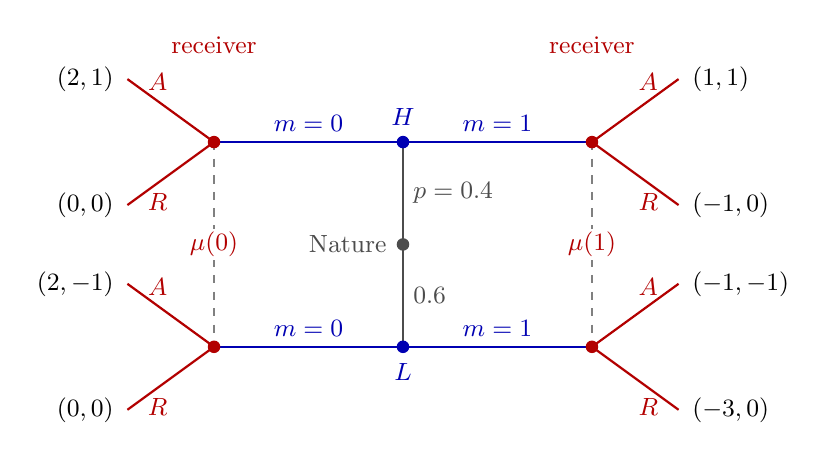
\begin{tikzpicture}[font=\small, >={Latex[length=2mm]},
    dec/.style={circle, fill, inner sep=1.6pt}]
  % Nature
  \draw[thick, gray!60!black] (0,0) -- node[right] {$p=0.4$} (0,1.3);
  \draw[thick, gray!60!black] (0,0) -- node[right] {$0.6$} (0,-1.3);
  \node[dec, gray!60!black, label={[gray!60!black]left:Nature}] at (0,0) {};
  % sender
  \foreach \y/\t in {1.3/H, -1.3/L} {
    \draw[thick, blue!70!black] (0,\y) -- node[above] {$m=0$} (-2.4,\y);
    \draw[thick, blue!70!black] (0,\y) -- node[above] {$m=1$} (2.4,\y);
  }
  \node[dec, blue!70!black, label={[blue!70!black]above:$H$}] at (0,1.3) {};
  \node[dec, blue!70!black, label={[blue!70!black]below:$L$}] at (0,-1.3) {};
  % receiver actions: A (outward and up), R (outward and down)
  \foreach \s in {-1,1} {
    \foreach \y in {1.3,-1.3} {
      \draw[thick, red!70!black] (\s*2.4,\y) -- node[pos=0.65, above] {$A$} (\s*3.5,\y+0.8);
      \draw[thick, red!70!black] (\s*2.4,\y) -- node[pos=0.65, below] {$R$} (\s*3.5,\y-0.8);
    }
  }
  % receiver information sets
  \draw[thick, dashed, gray] (-2.4,1.3) -- (-2.4,-1.3);
  \draw[thick, dashed, gray] (2.4,1.3) -- (2.4,-1.3);
  \node[red!70!black, fill=white, inner sep=1pt] at (-2.4,0) {$\mu(0)$};
  \node[red!70!black, fill=white, inner sep=1pt] at (2.4,0) {$\mu(1)$};
  \foreach \x in {-2.4, 2.4} \foreach \y in {1.3,-1.3} \node[dec, red!70!black] at (\x,\y) {};
  \node[red!70!black, anchor=south] at (-2.4,2.3) {receiver};
  \node[red!70!black, anchor=south] at (2.4,2.3) {receiver};
  % payoffs (sender, receiver)
  \node[anchor=east] at (-3.55,2.1) {$(2,1)$};
  \node[anchor=east] at (-3.55,0.5) {$(0,0)$};
  \node[anchor=east] at (-3.55,-0.5) {$(2,-1)$};
  \node[anchor=east] at (-3.55,-2.1) {$(0,0)$};
  \node[anchor=west] at (3.55,2.1) {$(1,1)$};
  \node[anchor=west] at (3.55,0.5) {$(-1,0)$};
  \node[anchor=west] at (3.55,-0.5) {$(-1,-1)$};
  \node[anchor=west] at (3.55,-2.1) {$(-3,0)$};
\end{tikzpicture}
\end{document}
